\documentclass{beamer}
\usepackage[utf8]{inputenc}

\usetheme{Madrid}
\usecolortheme{default}
\usepackage{amsmath,amssymb,amsfonts,amsthm}
\usepackage{txfonts}
\usepackage{multicol}
\usepackage{tkz-euclide}
\usepackage{listings}
\usepackage{adjustbox}
\usepackage{array}
\usepackage{tabularx}
\usepackage{gvv}
\usepackage{lmodern}
\usepackage{circuitikz}
\usepackage{tikz}
\usepackage{graphicx}
\usepackage{hyperref}
\usepackage{siunitx}

\setbeamertemplate{page number in head/foot}[totalframenumber]

\usepackage{tcolorbox}
\tcbuselibrary{minted,breakable,xparse,skins}



\definecolor{bg}{gray}{0.95}
\DeclareTCBListing{mintedbox}{O{}m!O{}}{%
  breakable=true,
  listing engine=minted,
  listing only,
  minted language=#2,
  minted style=default,
  minted options={%
    linenos,
    gobble=0,
    breaklines=true,
    breakafter=,,
    fontsize=\small,
    numbersep=8pt,
    #1},
  boxsep=0pt,
  left skip=0pt,
  right skip=0pt,
  left=25pt,
  right=0pt,
  top=3pt,
  bottom=3pt,
  arc=5pt,
  leftrule=0pt,
  rightrule=0pt,
  bottomrule=2pt,
  toprule=2pt,
  colback=bg,
  colframe=orange!70,
  enhanced,
  overlay={%
    \begin{tcbclipinterior}
    \fill[orange!20!white] (frame.south west) rectangle ([xshift=20pt]frame.north west);
    \end{tcbclipinterior}},
  #3,
}
\lstset{
    language=C,
    basicstyle=\ttfamily\small,
    keywordstyle=\color{blue},
    stringstyle=\color{orange},
    commentstyle=\color{green!60!black},
    numbers=left,
    numberstyle=\tiny\color{gray},
    breaklines=true,
    showstringspaces=false,
}
%------------------------------------------------------------
%This block of code defines the information to appear in the
%Title page
\title %optional
{12.434}
\date{October 12,2025}
%\subtitle{A short story}

\author % (optional)
{Aditya Appana - EE25BTECH11004}

\begin{document}


\frame{\titlepage}
\begin{frame}{Question}
The two sides of a parallelogram are given by the vectors $\vec{A}= 2\hat{i} - 3\hat{j}$ and $\vec{B} = 3\hat{i} + 2\hat{j}.$
The area of the parallelogram is:
\end{frame}



\begin{frame}[fragile]
    \frametitle{Solution}
Let:
\begin{align}
    \vec{a} = \myvec{2\\-3\\0}\\
    \vec{b} = \myvec{3\\2\\0}
\end{align}\\
\end{frame}



\begin{frame}[fragile]
    \frametitle{Solution}
The area of the parallelogram can be expressed as:
\begin{align}
\vec{a}\times\vec{b}=
\myvec{|\vec{A_{23}} \vec{B_{23}}| \\ |\vec{A_{31}}   \vec{B_{31}}| \\ |\vec{A_{12}} \vec{B_{12}}| }
\end{align}
Substituting values:
\begin{align}
   \vec{a}\times\vec{b}= \myvec{0\\0\\13}
\end{align}
\end{frame}


\begin{frame}[fragile]
\frametitle{Solution}
Therefore, the area of the parallelogram is:
\begin{align}
\norm{\vec{a}\times\vec{b}}  = 13
\end{align}
It can be seen that $\vec{a}$ and $\vec{b}$ are orthogonal, and $\norm{\vec{a}} = \norm{\vec{b}}$, therefore they form the sides of a square.\\
Therefore the area can also be calculated as:
\begin{align}
    {\norm{\vec{a}}}^2 = ({\sqrt{13}})^2 = 13
\end{align}
\end{frame}

\begin{frame}[fragile]
    \frametitle{Code}
    \href{https://github.com/AdityaAppana/ee1030-2025/tree/553c177f5198dba6374b2aaed046a7bb580bf421/ee25btech11004/matgeo/12.434/Codes}{Codes permalink}

\end{frame}

\begin{frame}[fragile]
    \frametitle{Figure}
\begin{figure}[H]
    \centering
    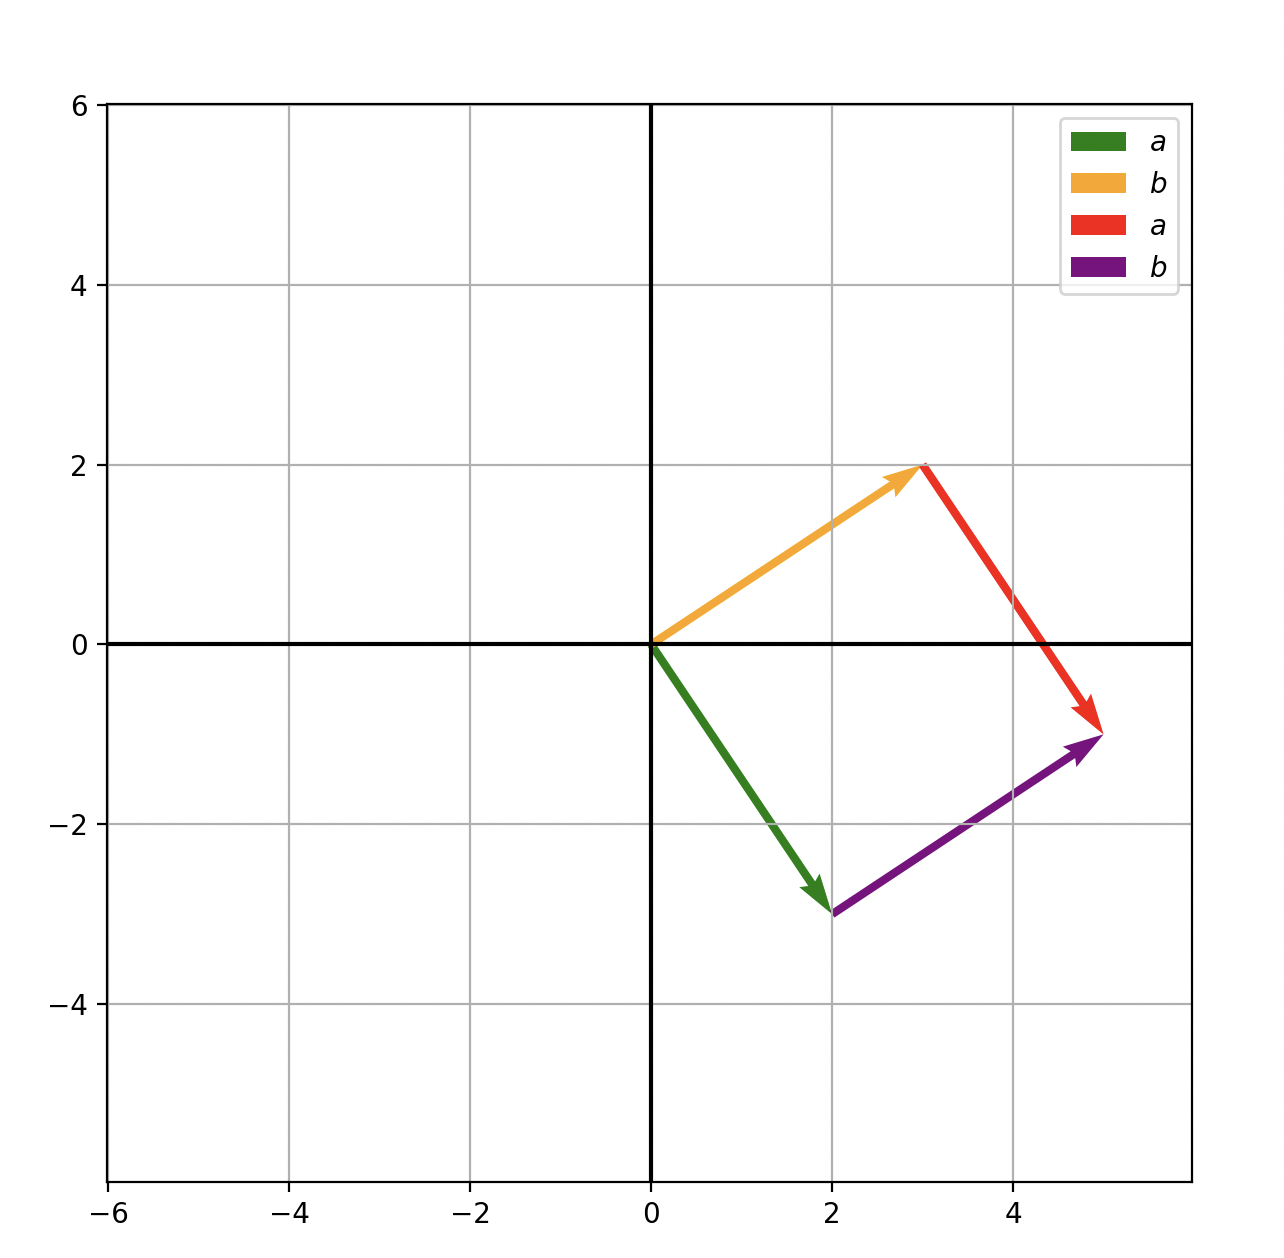
\includegraphics[width=0.6\columnwidth]{Figs/12434.png}
    \caption{Plot}
    \label{fig:placeholder}
\end{figure}
\end{frame}

\end{document}
